\documentclass[a4paper,sffamily,12pt]{article}

\usepackage[T1]{fontenc}
\usepackage[french]{babel}
\usepackage[utf8]{inputenc}

% Customization des listes
\usepackage{enumitem}
\usepackage{pifont}

% Insertion d'image
\usepackage{graphicx}

% Création de lien
\usepackage[colorlinks,linkcolor=blue]{hyperref}

% Formatage des titres de sections
\usepackage{titlesec}
\titleformat{\section}
  {\normalfont\Large\bfseries\sffamily}{\thesection.}{0.33em}{}[\hrule]
\titleformat{\paragraph}
  {\normalfont\bfseries\sffamily}{\theparagraph.}{0.33em}{}
 
 % tableau rectangle 
%\usepackage{slashbox}
%\usepackage{tabularx}

 % En-tête
\usepackage{fancyhdr}
\pagestyle{fancy}
\renewcommand\headrulewidth{1pt}
\fancyhead[L]{Base de données évoluées}
\fancyhead[R]{$X1I1050$}

% Permet de mettre du texte au dessus du titre
\usepackage{titling}
\renewcommand{\maketitlehooka}{\noindent COUILLEROT Carol \hfill  \hfill \\ MAHIER Loïc \hfill \\ PHALAVANDISHVILI  Demetre}

% Titre
\title{\vspace{\fill}\LARGE\bfseries\sffamily Rapport de projet\protect\footnote{rapport réalisé sous \LaTeX} \vspace{\fill}}

\begin{document}

	\date{} % Supprime la date
	\maketitle % Affiche le titre

	\thispagestyle{fancy} % Permet de mettre le titre sur la page ''fancy''
	
	\newpage
			
	\renewcommand{\contentsname}{Sommaire}
	\tableofcontents
	
	\newpage
	
	\section{Introduction}

		\vspace{0.5cm}
		
		L'objectif de ce projet est de réaliser un entrepôt de données (OLAP) ainsi que des requêtes intéressantes sur un ou plusieurs jeu de données libres (open data). Pour ce faire nous avons choisis deux jeux de données. Nous avons également choisis de réaliser ce projet en PL/SQL ainsi que d'utiliser Talend pour nettoyer nos données et concevoir nos tables relationnelles. \\


	\section{Choix des données}				

		\vspace{0.5cm}
		
		 Nous avons trouver nos données sur le site ''opendatasoft'', elles sont aussi présente sur le site ''data.gouv''. Le premier jeu de données est sur les hébergements collectifs en France : c'est à dire les hôtels, les campings et les résidences avec des informations sur leur location, leur classement (étoile) et leur capacité d'accueil notamment. Le deuxième jeu de donnée recueil toutes les communes de France, en indiquant leur population, leur superficie, leur code postal ainsi que leur département et leur région entre autre. Ce dernier nous permet d'affiner nos requête, d'en proposer des plus complexes mais aussi de pouvoir faire des regroupements et des classements par région et par département. Nous allons ainsi pouvoir faire des requêtes sur le classement (en étoile) de ces hébergements par département et région. Nous pourrons aussi regarder par commune, le nombre d'hôtels par habitant ou bien même faire une comparaison du nombre d'hébergement par région en fonction de l'année. \\

		\vspace{0.5cm}
		
	\section{Constellation de faits}

		\vspace{0.5cm}
			
		Après avoir choisis nos jeux de données, nous avons distinguer deux tables de faits : une propre aux hébergements avec des information sur leur capacité d'accueil et leur classement par exemple. Et une seconde propre aux communes, avec leur population, leur superficie et leur location (département, région). Pour pouvoir faire des requêtes intéressantes et donc pour pouvoir joindre nos deux tables de faits, nous utilisons l'identifiant de l'établissement (de l'hébergement) qui est présent dans les deux tables de faits. Cela nous permet ainsi d'accéder au caractéristiques propre à l'hébergement ainsi que celles propres à la commune de cette hébergement. Pour des raisons pratiques nous avons également choisis de faire une vue précise sur la location. Celle-ci nous affiche pour chaque commune, son code postale, son code INSEE, son département et sa région. Cette vue simplifiera nos requêtes complexes, d'autant que nous l'utiliserons fréquemment. ( ?? d'où le fait de l’indexer ?? )) \\
	
		\vspace{0.5cm}
		
		\begin{figure}[!h]
				
			\centerline{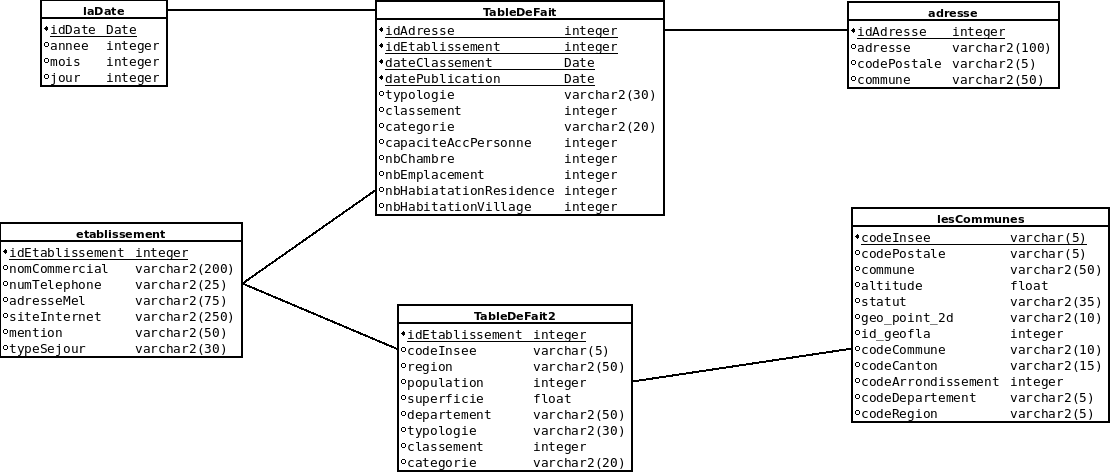
\includegraphics[height=8cm]{picture/constellation_de_fait.png}}
			\caption{La constellation de fait qui structure notre entrepôt de données}
			\label{constellation}
			
		\end{figure}	
		
		\vspace{0.5cm}
				
	\section{Intégration avec Talend}

		\vspace{0.5cm}
		
		
		
		
		
		
			
	\section{Requêtes}

		\vspace{0.5cm}
		
		
		
		
		
																
	\section{Conclusion}

		\vspace{0.5cm}
		
		
		
		
				

		\newpage
	
	\section{Annexe}
					
\end{document}
